\chapter{Time-memory-data tradeoff using Hellman tables}
\label{chapter:tmdto-hellman}

\paragraph{Summary}


\section{Hellman tables}
Time-memory tradeoff attacks were first conceived on block ciphers by Hellman in 1980. In this approach, Hellman proposed a method for carrying out the precomputation phase of the attack i.e. computing the precomputation tables. We refer to these tables as Hellman tables for block ciphers, in the remainder of the thesis. The proposed idea is based on the birthday paradox, and is thus probabilistic in nature, as we shall see in a moment. 

Later, using this approach as the basis, Shamir and Biryukov proposed a table structure for stream ciphers. This takes into account the amount of keystream available for the attack. We call these tables as Hellman tables for stream ciphers. We start by explaining the original idea of Hellman based on block ciphers. This is done by first presenting a naive approach to building tables for time-memory tradeoff attacks on block ciphers. Then, we point out limitations to the approach and explain how they are improved, consequently leading to the original idea of Hellman. From there, we provide the idea of Shamir and Biryukov, which is used for implementing a time-memory-data tradeoff attack on HiTag2 cipher. 

\subsection{Hellman tables for block ciphers}

A block cipher is an encryption algorithm, which takes in a plaintext block of $n$ bits (called the block size) and a key of $k$ bits, and returns the ciphertext block of $n$ bits. The following figure \ref{fig:block-cipher} illustrates a simple block cipher, with plaintext, ciphertext and key represented by $P$, $C$ and $K$ respectively. The encryption function is represented by $E$ such that $C$ = $E_K(P)$, implying encryption of $P$ under $K$.

\begin{figure}[ht!]
	\centering
		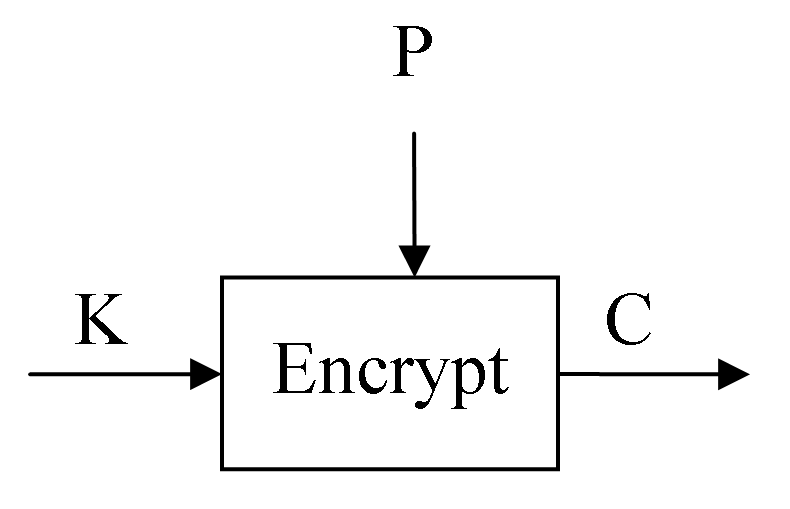
\includegraphics[width=2in]{./figures/block-cipher.PNG}
	\caption{A block cipher}	
	\label{fig:block-cipher}
\end{figure}

Consider the following scenario for a TMTO attack on block ciphers. The attacker has knowledge of a particular plaintext block $P$ and the corresponding ciphertext block $C$. The target is to find $K$, using which the attacker can decipher ciphertext for which the corresponding plaintext is not known. In addition, for simplicity, we assume the size of $K$ to be equal to the block size of $n$ bits. Then the precomputation and attack phases for a naive TMTO attack are explained.\\

\noindent \textit{\textbf{Naive attack: Precomputation phase.}} An $n$ bit value is randomly selected using a uniform distribution (and represented by $SP$ for a starting point). Using $SP$ as a key (denoted by $K_0$), encryption of $P$ is performed. The ciphertext obtained from this encryption is then used as the key (denoted by $K_1$) for another round of encryption of the same $P$. This procedure is iterated over a total of $t$ encryptions, yielding the key $K_t$ at the end. The key $K_t$ is called an end point, and is represented by $EP$. The sequence of encryptions starting from $SP$ to $EP$ is called a \emph{chain} and is illustrated in the figure \ref{fig:block-cipher-single-chain}. Equations for the $t$ encryptions are also shown below. 

\begin{center}
$K_0$ = $SP$\\
1. $K_1$ = $E_{K_0}(P)$\\
2. $K_2$ = $E_{K_1}(P)$\\
\vdots
$(t-1)$. $K_{t-1}$ = $E_{K_{t-2}}(P)$\\
$(t)$. $K_{t}$ = $E_{K_{t-1}}(P)$\\
$EP$ = $K_{t}$\\
\end{center}

\begin{figure}[ht!]
	\centering
		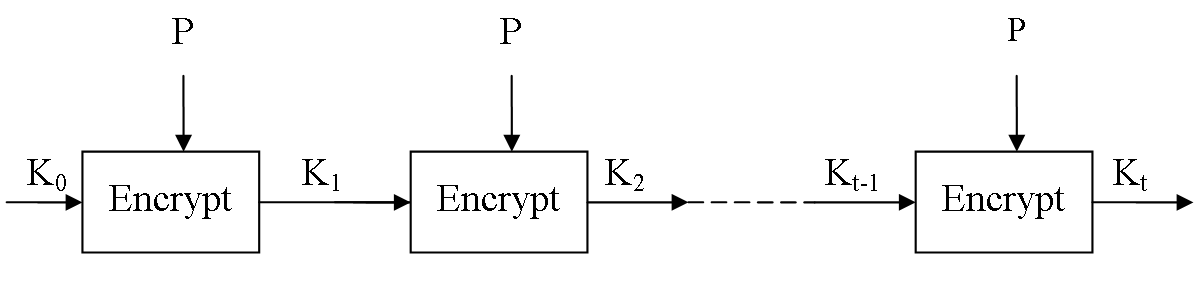
\includegraphics[width=5.5in]{./figures/block-cipher-single-chain.PNG}
	\caption{A chain of encryptions}	
	\label{fig:block-cipher-single-chain}
\end{figure}

In this fashion, a single chain is created. Note that though the chain contains a total of $(t+1)$ keys starting from $K_0$ to $K_{t}$, only the first $t$ keys are really useful during the attack phase. More on this is explained ahead. 

\begin{figure}[ht!]
	\centering
		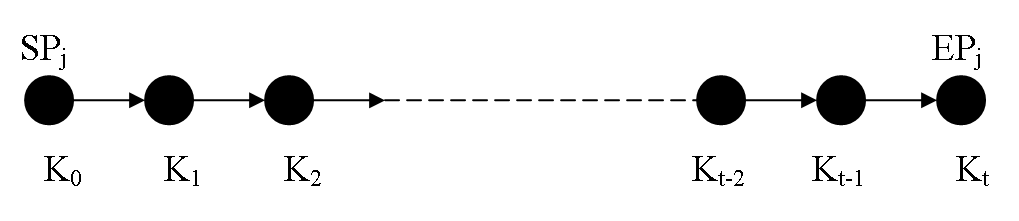
\includegraphics[width=4in]{./figures/single-chain.PNG}
	\caption{A single chain of encryptions represented by the pair $SP_j$ and $EP_j$}	
	\label{fig:single-chain}
\end{figure}

\begin{figure}[ht!]
	\centering
		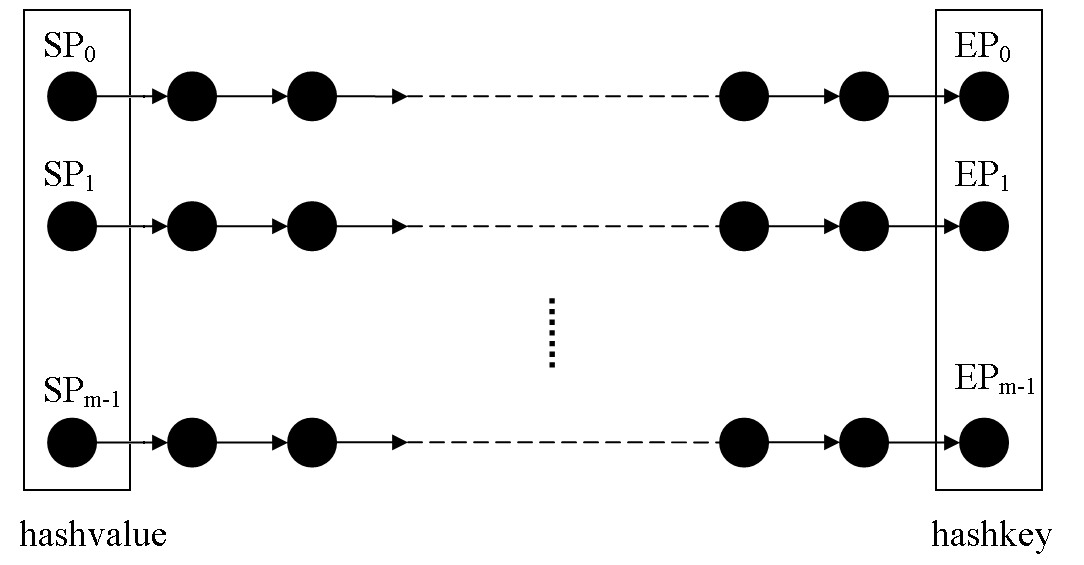
\includegraphics[width=4.5in]{./figures/naive-hellman-table.PNG}
	\caption{A naive precomputation table structure}	
	\label{fig:naive-hellman-table}
\end{figure}

During the precomputation phase, the goal is to cover the entire key space. An appropriate length of the chain is chosen so that no key repeats in the chain. Repetition is not desired since once a key reappears, subsequent keys also reappear, adding no extra information to the chain. Hence, the size of the chain is restricted, and more than one chains are created instead. 

Lets say $m$ more such chains are needed to cover all possible keys. If we consider the ideal case in which each chain contains $k$ distinct keys, then we have $m$ = $2^n/t$. For each chain, we select a random starting point $SP_j$ and end up with the end point $EP_j$, for $1 \leq j \leq m$, as shown in figure \ref{fig:single-chain}. Only the pairs $(SP_j,EP_j)$ are then stored in a hashtable, with $EP_j$ as the key and $SP_j$ as the corresponding value. All the chains representing such a naive table structure are illustrated in the figure \ref{fig:naive-hellman-table}.

We now compute $M$ and $P$ for such a table structure. The size of the memory required for storing all the chains would be of the order of $m$, as there are $m$ chains and a constant number of elements (two, precisely) corresponding to each chain are stored. Hence we have $M$ = $m$. Also, as there are $m.t$ encryptions performed in the entire table, the precomputation time $P$ = $m.t$.\\

\noindent  \textit{\textbf{Naive attack: Attack phase.}} If the key $K$ exists in the hashtable, the ciphertext $C$ would also exist. These possible locations of $K$ could be from $SP$ to $K_{t-2}$ for every chain. The $EP$ of every chain is not considered to be a possible key since it is not used in further encryption $P$. 

The first possibility is that $C$ lies in $(t-1)$'th column of one of the $m$ chains. If this is the case, then $K_{t-2}$ is the key we are looking for. To find this, we retrieve the corresponding $SP$ for that chain, and perform $(t-2)$ encryptions. After $(t-2)$ encryptions, $K_{t-2}$ is obtained. 

If $C$ does not match any $EP$ in the chains, the next possibility is that $C$ lies in the $(t-2)$'th column of some chain. To explore this possibility, we first evaluate $T$ = $E_{C}(P)$ and then match this value with the $EP$ for each chain. If there is a match, we know that the key $K_{t-3}$ is the required key. To find out $K_{t-3}$, we retrieve the $SP$ correspondng to the matched $EP$ and perform $(t-3)$ encryptions, at the end of which the output is $K_{t-3}$. If none of the $EP$ matches with the evaluated $T$, we explore the possibility of $C$ lying in the remaining columns. 




\subsection{Hellman tables for stream ciphers}


\section{Results from implementation}



%hellman tables for TMTO attacks on block ciphers
	% first proposal - then problems with it
	% second proposal in which we have multiple tables with different reduction functions
	

